\documentclass{beamer}
\usetheme{Boadilla}
\usecolortheme{sidebartab}
\beamertemplatenavigationsymbolsempty
\setbeamertemplate{footline}[frame number]
\usepackage{hyperref} 
\usepackage{graphicx}
\usepackage{color}
\usepackage{booktabs}
\usepackage{listings}
\usepackage{soul}
\usepackage{tikz}
\usepackage[utf8]{inputenc}

\definecolor{gray}{rgb}{0.4,0.4,0.4}
\definecolor{darkblue}{rgb}{0.0,0.0,0.6}
\definecolor{cyan}{rgb}{0.0,0.6,0.6}

\lstset{
	basicstyle=\ttfamily,
	columns=fullflexible,
	showstringspaces=false,
	commentstyle=\color{gray}\upshape
}

\lstdefinelanguage{XML}
{
	morestring=[b]",
	morestring=[s]{>}{<},
	morecomment=[s]{<?}{?>},
	stringstyle=\color{black},
	identifierstyle=\color{darkblue},
	keywordstyle=\color{cyan},
	morekeywords={xmlns,version,type}% list your attributes here
}

\makeatletter
\newcommand\SoulColor{%
	\let\set@color\beamerorig@set@color
	\let\reset@color\beamerorig@reset@color}
\makeatother

\lstset{language=XML}

\title{XML: Fortgeschrittene Themen}
\author{Markus Stocker}
\date{12. März 2018}

\begin{document}

\maketitle

\begin{frame}{Rekapitulation: Das ist ein ...}
	
	\texttt{<?xml version="1.0" encoding="utf-8"?>} \newline
	\texttt{<!-- Yet another example -->} \newline
	\texttt{<a:planets xmlns:a="http://astronomy.org">} \newline
	\texttt{<a:planet radius="6371 km">Earth</a:planet>} \newline
	\texttt{<a:planet><![CDATA[Mars]]></a:planet>} \newline
	\texttt{</a:planets>}
	
\end{frame}

\begin{frame}{Rekapitulation: Das ist eine ...}
	
	\SoulColor\hl{\texttt{<?xml version="1.0" encoding="utf-8"?>}} \newline
	\texttt{<!-- Yet another example -->} \newline
	\texttt{<a:planets xmlns:a="http://astronomy.org">} \newline
	\texttt{<a:planet radius="6371 km">Earth</a:planet>} \newline
	\texttt{<a:planet><![CDATA[Mars]]></a:planet>} \newline
	\texttt{</a:planets>}
	
\end{frame}

\begin{frame}{Rekapitulation: Das ist ein ...}
	
	\texttt{<?xml version="1.0" encoding="utf-8"?>} \newline
	\SoulColor\hl{\texttt{<!-- Yet another example -->}} \newline
	\texttt{<a:planets xmlns:a="http://astronomy.org">} \newline
	\texttt{<a:planet radius="6371 km">Earth</a:planet>} \newline
	\texttt{<a:planet><![CDATA[Mars]]></a:planet>} \newline
	\texttt{</a:planets>}
	
\end{frame}

\begin{frame}{Rekapitulation: Das ist ein ...}
	
	\texttt{<?xml version="1.0" encoding="utf-8"?>} \newline
	\texttt{<!-- Yet another example -->} \newline
	\SoulColor\hl{\texttt{<a:planets xmlns:a="http://astronomy.org">}} \newline
	\texttt{<a:planet radius="6371 km">Earth</a:planet>} \newline
	\texttt{<a:planet><![CDATA[Mars]]></a:planet>} \newline
	\texttt{</a:planets>}
	
\end{frame}

\begin{frame}{Rekapitulation: Das ist ein ...}
	
	\texttt{<?xml version="1.0" encoding="utf-8"?>} \newline
	\texttt{<!-- Yet another example -->} \newline
	\texttt{<a:planets \SoulColor\hl{xmlns:a="http://astronomy.org"}>} \newline
	\texttt{<a:planet radius="6371 km">Earth</a:planet>} \newline
	\texttt{<a:planet><![CDATA[Mars]]></a:planet>} \newline
	\texttt{</a:planets>}
	
\end{frame}

\begin{frame}{Rekapitulation: Das ist ein ...}
	
	\texttt{<?xml version="1.0" encoding="utf-8"?>} \newline
	\texttt{<!-- Yet another example -->} \newline
	\texttt{<a:planets xmlns:a="http://astronomy.org">} \newline
	\SoulColor\hl{\texttt{<a:planet radius="6371 km">Earth</a:planet>}} \newline
	\texttt{<a:planet><![CDATA[Mars]]></a:planet>} \newline
	\texttt{</a:planets>}
	
\end{frame}

\begin{frame}{Rekapitulation: Das ist ein ...}
	
	\texttt{<?xml version="1.0" encoding="utf-8"?>} \newline
	\texttt{<!-- Yet another example -->} \newline
	\texttt{<a:planets xmlns:a="http://astronomy.org">} \newline
	\texttt{<\SoulColor\hl{a:}planet radius="6371 km">Earth</a:planet>} \newline
	\texttt{<a:planet><![CDATA[Mars]]></a:planet>} \newline
	\texttt{</a:planets>}
	
\end{frame}

\begin{frame}{Rekapitulation: Das ist ein ...}
	
	\texttt{<?xml version="1.0" encoding="utf-8"?>} \newline
	\texttt{<!-- Yet another example -->} \newline
	\texttt{<a:planets xmlns:a="http://astronomy.org">} \newline
	\texttt{<a:planet \SoulColor\hl{radius="6371 km"}>Earth</a:planet>} \newline
	\texttt{<a:planet><![CDATA[Mars]]></a:planet>} \newline
	\texttt{</a:planets>}
	
\end{frame}

\begin{frame}{Rekapitulation: Das ist ...}
	
	\texttt{<?xml version="1.0" encoding="utf-8"?>} \newline
	\texttt{<!-- Yet another example -->} \newline
	\texttt{<a:planets xmlns:a="http://astronomy.org">} \newline
	\texttt{<a:planet radius="6371 km">Earth</a:planet>} \newline
	\texttt{<a:planet>\SoulColor\hl{<![CDATA[Mars]]>}</a:planet>} \newline
	\texttt{</a:planets>}
	
\end{frame}

\begin{frame}{Dieses XML Dokument ist nicht wohlgeformt weil ...}
	
	\texttt{<a:planets xmlns:a="http://astronomy.org">} \newline
	\texttt{<a:planet radius="6371 km">Earth < Mars</a:Planet>} \newline
	\texttt{<a:planet>![CDATA[Mars is ]]> next frontier]]></a:planets>} \newline
	\texttt{</a:planet>}
	\texttt{<!-- Yet another -- example -->} \newline
	
\end{frame}

\begin{frame}{Übersicht}
	
	\begin{itemize}
		\item XML Baumstruktur
		\item Sich auf einen Standard festlegen: Vokabularien in XML
		\item XML Vokabularien und Bedeutung
		\item XML in der Programmierung: Lesen, Schreiben, Verarbeiten
		\item XML und Datenbanken
		\item XML und Web Services
		\item Einige Nachteile von XML
	\end{itemize}
	
\end{frame}

\begin{frame}{Baumstruktur}
	
	\begin{itemize}
		\item Die Struktur der Elemente eines XML Dokumentes ergibt ein Baum
		\item Dokument enthält ein einziges \emph{root element}
		\item Das Element an der Spitze des Baumes
		\item Element kann ein oder mehrere ``Kindelemente'' (\emph{child}) enthalten
		\item Diese sind dem ``Elternelement'' (\emph{parent}) untergeordnet
	\end{itemize}
	
\end{frame}

\begin{frame}[fragile]{Baumstruktur}
	
	\begin{columns}[T] % align columns
		\begin{column}{.40\textwidth}
			\small
			\begin{lstlisting}
<planets>
  <planet>
    <name>Earth</name>
    <radius>6371</radius>
  </planet>
  <planet>
    <name>Mars</name>
  </planet>
</planets>
			\end{lstlisting}
		\end{column}%
		\hfill%
		\begin{column}{.55\textwidth}
			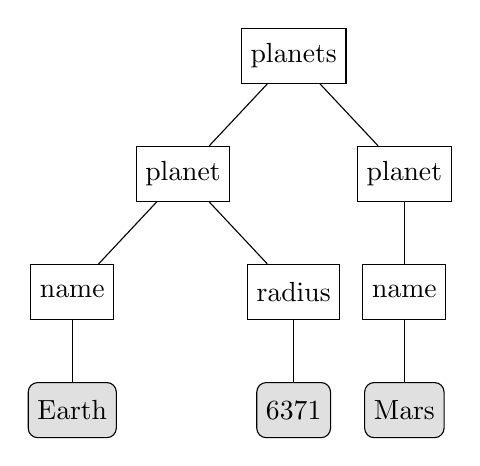
\begin{tikzpicture}[sibling distance=8em, node/.style = {shape=rectangle, draw, align=center, fill=white, minimum height=7mm}, leaf/.style = {shape=rectangle, draw, align=center, fill=gray!20, minimum height=7mm, rounded corners=.8ex}]
				\node[node]{planets}
				child { node[node]{planet} 
					child { node[node]{name} child { node[leaf]{Earth} } }
					child { node[node]{radius} child { node[leaf]{6371} } }
				}
				child { node[node]{planet}
					child { node[node]{name} child { node[leaf]{Mars} } }
				};
			\end{tikzpicture}
		\end{column}%
	\end{columns}
	
\end{frame}

\begin{frame}{Vokabularien in XML}
	
	\begin{itemize}
		\item Dass Daten in XML vorliegen bedeutet nicht, dass diese nützlich sind
		\item Programme A und B können Zeichnungen als XML speichern
		\item Bedeutet nicht, dass die Zeichnungen austauschbar sind
		\item Austauschbarkeit bedarf gemeinsame Festlegung auf ein Vokabular
		\item Auch ``Standard'' genannt, z.B. Scalable Vector Graphics (SVG)
	\end{itemize}
	
\end{frame}

\begin{frame}{Vokabularien in XML}
	
	\begin{itemize}
		\item Sich auf einen Vokabular festlegen bedeutet
		\item Entweder ein existierendes aufnehmen (z.B. einen Standard)
		\item Oder zumindest darauf aufbauen
		\item Oder aber mit der community ein Vokabular erstellen
	\end{itemize}
	
\end{frame}

\begin{frame}[fragile]{Vokabularien in XML}
	
	\begin{itemize}
		\item Wie man Daten in XML strukturiert ist entscheidend
		\item Eine Anwendung erwartet eine gewisse Struktur
		\item Anwendungen werden anhand einer Struktur entwickelt
	\end{itemize}
	
	\begin{columns}[T] % align columns
		\begin{column}{.52\textwidth}
			\begin{lstlisting}
<planets>
  <planet>
    <name>Earth</name>
    <radius>6371</radius>
  </planet>
</planets>
			\end{lstlisting}
		\end{column}%
		\hfill%
		\begin{column}{.44\textwidth}
			\begin{lstlisting}
<planets>
  <planet name="Earth" 
           radius="6371" 
  />
</planets>
			\end{lstlisting}
		\end{column}%
	\end{columns}
	
\end{frame}

\begin{frame}{Vokabularien in XML}
	
	\begin{itemize}
		\item \emph{Tags} haben für Software keinerlei Bedeutung
		\item Ob \texttt{<planet>Earth</planet>} oder \texttt{<x>Earth</x>}
		\item Für Software macht dies kein (grosser) Unterscheid
		\item Nur die Baumstruktur ist für die Software von Bedeutung
		\item Selbstbeschreibend ist XML also hauptsächlich für Menschen
		\item Jedoch ist XML selbst für Menschen oft nicht einfach zu verstehen
		\item Weil die Bedeutung der \emph{tags} oft nicht klar ist
	\end{itemize}
	
\end{frame}

\begin{frame}{XML in der Programmierung: Lesen und Schreiben}
	
	\begin{itemize}
		\item XML ist in gängigen Programmiersprachen les- und schreibar
		\item Und zwar aus den verschiedesten Sourcen
		\item Lesen aus \texttt{string} haben wir bereits gesehen
		\item Möglich ist auch das Lesen und Schreiben aus/zu 
		\begin{itemize}
			\item Dateien
			\item Datenbanken
			\item Internet
		\end{itemize}
	\end{itemize}
	
\end{frame}

\begin{frame}[fragile]{XML in der Programmierung: Programmatisch Schreiben}
	
	\lstset{language=Python}
	\scriptsize
	\begin{lstlisting}
from lxml import etree as et

planets = et.Element('planets')
planet_earth = et.SubElement(planets, 'planet')
planet_mars = et.SubElement(planets, 'planet')
earth_name = et.SubElement(planet_earth, 'name')
earth_radius = et.SubElement(planet_earth, 'radius')
mars_name = et.SubElement(planet_mars, 'name')
earth_name.text = 'Earth'
earth_radius.text = '6371'
mars_name.text = 'Mars'

print(et.tostring(planets, pretty_print=True).decode('utf-8'))

<planets>
  <planet>
    <name>Earth</name>
    <radius>6371</radius>
  </planet>
  <planet>
    <name>Mars</name>
  </planet>
</planets>
	\end{lstlisting}
	
\end{frame}

\begin{frame}{XML in der Programmierung: Verarbeiten}
	
	\begin{itemize}
		\item Einmal gelesen, kann XML programmatisch verarbeitet werden
		\item Programmiersprachen stellen dafür Funktionalität zur Verfügung
		\item Diese erlaubt das Durchlaufen des Baumes
		\item Wie auch der geziehlte Zugriff auf Elemente, Attribute, etc.
	\end{itemize}
	
\end{frame}

\begin{frame}[fragile]{XML in der Programmierung: Verarbeiten}

	\lstset{language=Python}
	\scriptsize
	\begin{lstlisting}
from lxml import etree as et

planets = et.fromstring("""
  <planets>
    <planet>
      <name>Earth</name>
      <radius>6371</radius>
    </planet>
    <planet>
      <name>Mars</name>
    </planet>
  </planets>
""")

for planet in planets:
  for quality in planet:
    print('{}: {}'.format(quality.tag, quality.text))
    
name: Earth
radius: 6371
name: Mars
	\end{lstlisting}
	
\end{frame}

\begin{frame}{XML und Datenbanken}
	
	\begin{itemize}
		\item Datenbank die XML Dokumente speichern und durchsuchen zu kann
		\item Dokumentenorientierten Datenbank (NoSQL)
		\item Underscheidet sich von relationalen Datenbankmodellen
		\item XPath, XQuery, XSL zur Abfrage und Manipulation verwendet
		\item Native XML-Datenbanksysteme: BaseX, Berkeley DB XML, etc.
		\item XML-enabled Datenbanken: IBM, Oracle, Microsoft
	\end{itemize}
	
\end{frame}

\begin{frame}{XML und Web Services}
	
	\begin{itemize}
		\item XML besonders im Internet Datenaustausch verbreitet
		\item Viele Web Services and Web API liefern Daten in XML
		\item Allerdings nimmt die Bedeutung anderer Formate zu (z.B. JSON)
	\end{itemize}
	
\end{frame}

{
	\usebackgroundtemplate{ %
		\begin{tikzpicture}[remember picture, overlay]%
		\node at (current page.center) {\includegraphics[width=.9\paperwidth]{xml-json.png}};%
		\end{tikzpicture}%
	}%
	\setbeamertemplate{navigation symbols}{}
	\begin{frame}[plain]
		\vspace{7cm}
		\begin{center}
Google Trends: XML (blau) und JSON (rot), seit 2008
		\end{center}
	\end{frame}
}

\begin{frame}[fragile]{XML und Web Services}
	
	\lstset{language=Python}
	\scriptsize
	\begin{lstlisting}
import requests
	
url = '{}?verb={}&metadataPrefix={}&identifier={}'.format(
	'http://ws.pangaea.de/oai/provider',
	'GetRecord', 
	'datacite3', 
	'oai:pangaea.de:doi:10.1594/PANGAEA.858171'
)
	
r = requests.get(url)
	
x = et.XML(bytes(bytearray(r.text, 'utf-8')))
	
print(x.find(
  './/{http://datacite.org/schema/kernel-3}identifier[@identifierType="DOI"]'
  ).text)
 
10.1594/PANGAEA.858171
	\end{lstlisting}
	
\end{frame}


\begin{frame}{Einige Nachteile von XML}
	
	\begin{itemize}
		\item Das \texttt{tagging} ist ``Ballast''
		\item Speziell bei stark regulären Daten (z.B. Tabellen) 
		\item Grosser Speicherbedarf und Bandbreite
		\item Problematisch wenn diese fehlen, z.B. Sensordaten
	\end{itemize}
	
\end{frame}

\begin{frame}{Zusammenfassung}
	
	\begin{itemize}
		\item
	\end{itemize}
	
\end{frame}

\end{document}